\begin{center}
    \begin{large}
    CP 1 - Operaciones básicas\\
    Curso \academicyear\\
    \end{large}
    
\begin{figure}[h]
    \centering
    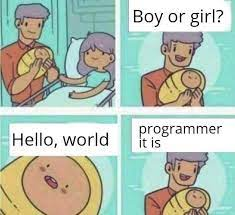
\includegraphics[width=0.4\linewidth]{cp2/hello_world.jpg}
\end{figure}
\end{center}

% Basic
\section{Di hola}
\begin{enumerate}
	\item Muestre en la consola el siguiente string: "Hello, World!".
	\item Muestre en la consola el valor máximo y el valor mínimo admitidos por el tipo $int$.
	\item Muestre en la consola un valor aproximado de Pi (use la clase $Math$).
\end{enumerate}
\ifshowanswers
\section*{Respuesta:}
\begin{enumerate}
	\item Muestre en la consola el siguiente string: "Hello, World!".
        \begin{lstlisting}
    Console.WriteLine("Hello, World!");
        \end{lstlisting}
	\item Muestre en la consola el valor máximo y el valor mínimo admitidos por el tipo $int$.
        \begin{lstlisting}
    Console.WriteLine($"Valor máximo de int: {int.MaxValue}");
    Console.WriteLine($"Valor mínimo de int: {int.MinValue}");
        \end{lstlisting}
	\item Muestre en la consola un valor aproximado de Pi (use la clase $Math$).
         \begin{lstlisting}
    Console.WriteLine($"Pi: {Math.PI}");
        \end{lstlisting}
\end{enumerate}
\fi

\section{Doble}
Escribe un programa que lea de la consola un número entero y muestre en la consola su doble.
\subsection*{Ejemplos}
\begin{itemize}
    \item Entrada: \texttt{4}\\
          Salida: \texttt{8}
    \item Entrada: \texttt{-5}\\
          Salida: \texttt{-10}
    \item Entrada: \texttt{0}\\
          Salida: \texttt{0}
\end{itemize}
\ifshowanswers
\section*{Respuesta:}
\begin{lstlisting}
    //Solicitar al usuario que ingrese un número entero
    Console.Write("Ingrese un número entero: ");
        
    // Leer el número ingresado por el usuario
    int number = Convert.ToInt32(Console.ReadLine());
        
    // Calcular el doble del número
    int doble = number * 2;
        
    // Mostrar el resultado en la consola
    Console.WriteLine($"El doble de {number} es {double}");
\end{lstlisting}

\fi

\section{Área de un triángulo}
Escribe un programa que lea de la consola la base \(b\) y la altura \(h\) de un triángulo, calcule su área y la escriba en la consola.\\
\[
\text{Área} = \frac{b \cdot h}{2}
\]
\subsection*{Ejemplos}
\begin{itemize}
    \item Entrada: \texttt{b = 10, h = 5}\\
          Salida: \texttt{Área = 25}
    \item Entrada: \texttt{b = 3, h = 4}\\
          Salida: \texttt{Área = 6}
\end{itemize}

\section{Promedio de tres números}
Escribe un programa que lea tres números reales \(x\), \(y\) y \(z\) de la consola, calcule su promedio y lo muestre en la consola.
\subsection*{Ejemplos}
\begin{itemize}
    \item Entrada: \texttt{3.0, 4.0, 5.0}\\
          Salida: \texttt{Promedio = 4.0}
    \item Entrada: \texttt{-1.0, -2.0, -3.0}\\
          Salida: \texttt{Promedio = -2.0}
    \item Entrada: \texttt{10.5, 20.5, 30.5}\\
          Salida: \texttt{Promedio = 20.5}
\end{itemize}

\section{Cambio de temperatura}
Escribe un programa que lea de la consola una temperatura en grados Fahrenheit (\(F\)), la convierta a grados Celsius (\(C\)) y muestre el resultado en la consola.\\ 
\[
C = \frac{5}{9} \cdot (F - 32)
\]
\subsection*{Ejemplos}
\begin{itemize}
    \item Entrada: \texttt{F = 50}\\
          Salida: \texttt{C = 10}
    \item Entrada: \texttt{F = 32}\\
          Salida: \texttt{C = 0}
    \item Entrada: \texttt{F = 96.8}\\
          Salida: \texttt{C = 36}
\end{itemize}

\section{Perímetro y área de un círculo}
Escribe un programa que lea de la consola el radio \(r\) de un círculo, calcule su perímetro y su área, y muestre ambos resultados en la consola.\\   
\[
\text{Perímetro} = 2\pi r, \quad \text{Área} = \pi r^2
\]
\subsection*{Ejemplos}
\begin{itemize}
    \item Entrada: \texttt{r = 3}\\
          Salida: \texttt{Perímetro = 18.8496, Área = 28.2744}
    \item Entrada: \texttt{r = 0}\\
          Salida: \texttt{Perímetro = 0, Área = 0}
    \item Entrada: \texttt{r = 1.5}\\
          Salida: \texttt{Perímetro = 9.4248, Área = 7.0686}
\end{itemize}

\section{Hipotenusa}
Escribe un programa que lea de la consola los catetos \(a\) y \(b\) de un triángulo rectángulo, calcule la longitud de su hipotenusa y la escriba en la consola.\\
\[
c = \sqrt{a^2 + b^2}
\]
\subsection*{Ejemplos}
\begin{itemize}
    \item Entrada: \texttt{a = 3, b = 4}\\
          Salida: \texttt{c = 5}
    \item Entrada: \texttt{a = 5, b = 12}\\
          Salida: \texttt{c = 13}
    \item Entrada: \texttt{a = 8, b = 15}\\
          Salida: \texttt{c = 17}
\end{itemize}

% Intermediate
\section{Suma de dígitos}
Escribe un programa que lea un número entero de tres cifras \(n\) de la consola, calcule la suma de sus dígitos y la muestre en la consola.\\
Ejemplo: Si \(n = 123\), entonces:
\[
\text{suma} = 1 + 2 + 3
\]
Pista: Usa la división y resto de la división para extraer los dígitos:
\[
\text{Centena} = \frac{n}{100}, \quad \text{Decena} = \frac{(n \% 100)}{10}, \quad \text{Unidad} = n \% 10
\]
\subsection*{Ejemplos}
\begin{itemize}
    \item Entrada: \texttt{n = 123}\\
          Salida: \texttt{Suma = 6}
    \item Entrada: \texttt{n = 456}\\
          Salida: \texttt{Suma = 15}
    \item Entrada: \texttt{n = 789}\\
          Salida: \texttt{Suma = 24}
\end{itemize}

\section{Ecuación cuadrática}
Reciba los coeficientes \(a\), \(b\) y \(c\) (números reales) de una ecuación cuadrática de la forma:

\[
ax^2 + bx + c = 0
\]

y, asumiendo que la ecuación tiene dos soluciones reales, calcule las raíces de la ecuación utilizando la fórmula cuadrática:

\[
x = \frac{-b \pm \sqrt{b^2 - 4ac}}{2a}
\]

Se asegura que el discriminante (\(\Delta = b^2 - 4ac\)) es mayor que 0 para que existan dos soluciones reales.

\subsection*{Ejemplos}
\begin{itemize}
    \item Entrada: \texttt{a = 1, b = -3, c = 2}\\
          Salida: \texttt{x1 = 2, x2 = 1}
    \item Entrada: \texttt{a = 2, b = 5, c = -3}\\
          Salida: \texttt{x1 = 0.5, x2 = -3}
    \item Entrada: \texttt{a = 1, b = -6, c = 8}\\
          Salida: \texttt{x1 = 4, x2 = 2}
\end{itemize}

\ifshowanswers
\section*{Respuesta:}
Para la ecuación cuadrática, las soluciones son:

$$
x_1 = \frac{-b + \sqrt{D}}{2a}
$$

y

$$
x_2 = \frac{-b - \sqrt{D}}{2a}
$$

donde

$$D = b^2 - 4ac$$

Esta fórmula nos da las soluciones de la ecuación cuadrática, siempre y cuando el discriminante sea mayor o igual a cero.

\begin{lstlisting}
    Console.WriteLine("Ingrese el coeficiente a:");
    double a = double.Parse(Console.ReadLine());
    
    Console.WriteLine("Ingrese el coeficiente b:");
    double b = double.Parse(Console.ReadLine());
    
    Console.WriteLine("Ingrese el coeficiente c:");
    double c = double.Parse(Console.ReadLine());
    
    double discriminant = b * b - 4 * a * c;
    
    double x1 = (-b + Math.Sqrt(discriminant)) / (2 * a);
    double x2 = (-b - Math.Sqrt(discriminant)) / (2 * a);
    
    Console.WriteLine($"Las soluciones son x1 = {x1} y x2 = {x2}"
\end{lstlisting}
\fi

\section{Distancia entre dos puntos}
Escribe un programa que lea de la consola las coordenadas de dos puntos \( (x_1, y_1) \) y \( (x_2, y_2) \) en el plano, calcule la distancia entre ellos y escriba el resultado en la consola.\\
\[
\text{Distancia} = \sqrt{(x_2 - x_1)^2 + (y_2 - y_1)^2}
\]
\subsection*{Ejemplos}
\begin{itemize}
    \item Entrada: \texttt{(x1 = 1, y1 = 2), (x2 = 4, y2 = 6)}\\
          Salida: \texttt{Distancia = 5}
    \item Entrada: \texttt{(x1 = 0, y1 = 0), (x2 = 3, y2 = 4)}\\
          Salida: \texttt{Distancia = 5}
    \item Entrada: \texttt{(x1 = -1, y1 = -1), (x2 = 2, y2 = 3)}\\
          Salida: \texttt{Distancia = 5}
\end{itemize}

% Advanced
\section{Minutos a horas}
Escribe un programa que lea un número entero \(t\) que representa una cantidad de minutos de la consola, calcule cuántas horas completas y cuántos minutos sobran, y muestre ambos valores en la consola.\\
\textbf{Pista:} Usa la división y resto de la división para manejar cuando te pases de 60:
\[
\text{Horas} = \frac{t}{60}, \quad \text{Minutos} = t \% 60
\]
\subsection*{Ejemplos}
\begin{itemize}
\item Entrada: \texttt{t = 130}\\
      Salida: \texttt{Horas = 2, Minutos = 10}
\item Entrada: \texttt{t = 75}\\
      Salida: \texttt{Horas = 1, Minutos = 15}
\item Entrada: \texttt{t = 45}\\
      Salida: \texttt{Horas = 0, Minutos = 45}
\end{itemize}

\section{Mayor}
Reciba dos números enteros de la consola y determine cuál de los dos es mayor sin utilizar $Math.Max$ y $Math.Min$. No utilice condicionales.
\subsection*{Ejemplos}
\begin{itemize}
\item Entrada: \texttt{a = 5, b = 10}\\
      Salida: \texttt{Mayor = 10}
\item Entrada: \texttt{a = -3, b = -7}\\
      Salida: \texttt{Mayor = -3}
\item Entrada: \texttt{a = 12, b = 12}\\
      Salida: \texttt{Mayor = 12}
\end{itemize}

\section{Valor medio}
Reciba tres números enteros. Muestre en la consola el de valor medio (Utilice $Math.Max$ y $Math.Min$) y el promedio de estos.
\subsection*{Ejemplos}
\begin{itemize}
    \item Entrada: \texttt{a = 5, b = 10, c = 15}\\
        Salida: \texttt{Valor medio = 10, Promedio = 10}
    \item Entrada: \texttt{a = -3, b = 4, c = 8}\\
        Salida: \texttt{Valor medio = 4, Promedio = 3}
    \item Entrada: \texttt{a = 7, b = 7, c = 7}\\
        Salida: \texttt{Valor medio = 7, Promedio = 7}
\end{itemize}
    
\section{Intercambio de variables}
Dado que tienes dos enteros guardados en las variables \(a\) y \(b\), realiza el intercambio de sus valores de las siguientes maneras:

\begin{enumerate}
    \item Usando una variable auxiliar.
    \item Sin usar una variable auxiliar.
\end{enumerate}

\subsection*{Ejemplo:} 
Supongamos que las variables inicializan de la siguiente manera:
\begin{lstlisting}
    int a = 5;
    int b = 9;
\end{lstlisting}

si al final de tu programa  añades la línea:
\begin{lstlisting}
    Console.WriteLine($"El valor de a es {a} y el valor de b es {b}.");
\end{lstlisting}

La salida esperada en la consola es:
\begin{verbatim}
    El valor de a es 9 y el valor de b es 5.
\end{verbatim}

\ifshowanswers
\section*{Respuesta:}
\textbf{Usando una variable auxiliar:}
\begin{lstlisting}
    Console.WriteLine("Ingrese dos números enteros:");
    int a = int.Parse(Console.ReadLine());
    int b = int.Parse(Console.ReadLine());
    
    int temp = a;
    a = b;
    b = temp;
    
    Console.WriteLine($"El valor de a es {a} y el valor de b es {b}.");
\end{lstlisting}

\textbf{Usando operaciones aritméticas:}
\begin{lstlisting}
    Console.WriteLine("Ingrese dos números enteros:");
    int a = int.Parse(Console.ReadLine());
    int b = int.Parse(Console.ReadLine());
    
    // Valores iniciales: a = x, b = y
    // Paso 1: Sumar ambos números y almacenar el resultado en 'a'
    a += b;
    // Ahora, a = x + y, b = y
    
    // Paso 2: Restar el nuevo valor de 'a' (que es x + y) por 'b' (que es y)
    // Esto nos da el valor original de 'a' (que es x) y lo almacena en 'b'
    b = a - b;
    // Ahora, b = x, a = x + y
    
    // Paso 3: Restar el nuevo valor de 'b' (que es x) de 'a' (que es x + y)
    // Esto nos da el valor original de 'b' (que es y) y lo almacena en 'a'
    a -= b;
    // Ahora, a = y, b = x
    
    // En este punto, los valores de 'a' y 'b' han sido intercambiados
    Console.WriteLine($"El valor de a es {a} y el valor de b es {b}.");
\end{lstlisting}
\fi

\section{Circunferencias}
Sean las circunferencias $C_1$ y $C_2$ de redio $r$. Lea de la consola el radio $r$ (puede ser cualquier número real, no solo entero) y calcule el área sombreada.

\begin{center}
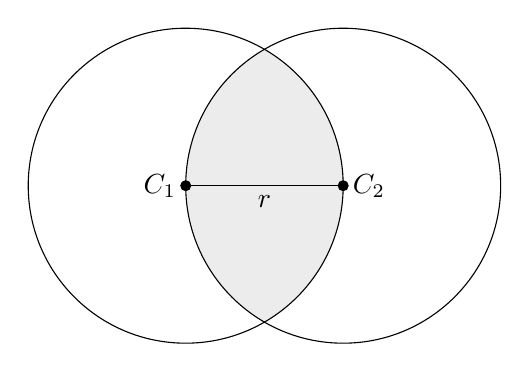
\begin{tikzpicture}
    % Definir el radio
    \def\r{2}

    % Sombrear el área de intersección
    \begin{scope}
        \clip (0,0) circle (\r);
        \fill[gray!15] (\r,0) circle (\r);
    \end{scope}

    % Dibujar la primera circunferencia
    \draw (0,0) circle (\r);

    % Dibujar la segunda circunferencia con un radio coincidente
    \draw (\r,0) circle (\r);

    % Marcar los centros de las circunferencias
    \fill (0,0) circle (2pt) node[left] {$C_1$};
    \fill (\r,0) circle (2pt) node[right] {$C_2$};

    % Dibujar el radio coincidente y etiquetarlo
    \draw (0,0) -- (\r,0) node[midway, below] {$r$};
\end{tikzpicture}
\end{center}

\subsection*{Ejemplos}
\begin{itemize}
    \item Entrada: \texttt{3}\\
          Salida: \texttt{El área sombreada es: 18.84955592153876}
    \item Entrada: \texttt{5}\\
          Salida: \texttt{El área sombreada es: 52.35987755982988}
    \item Entrada: \texttt{10}\\
          Salida: \texttt{El área sombreada es: 209.43951023931953}
\end{itemize}

\ifshowanswers
\section*{Respuesta:}
Vamos a nombrar P a uno de los puntos de intersección de las circunferencias y vamos a trazar los siguientes radios:

\begin{center}
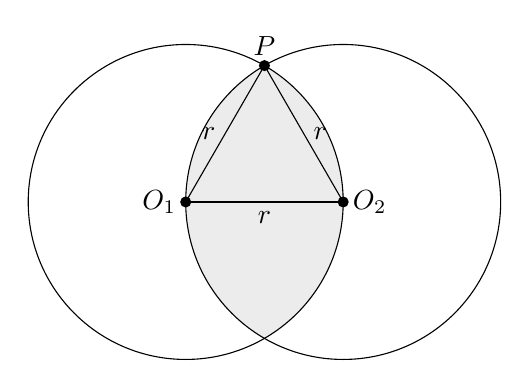
\begin{tikzpicture}
    % Definir el radio
    \def\r{2}

    % Sombrear el área de intersección
    \begin{scope}
        \clip (0,0) circle (\r);
        \fill[gray!15] (\r,0) circle (\r);
    \end{scope}

    % Dibujar la primera circunferencia
    \draw (0,0) circle (\r);

    % Dibujar la segunda circunferencia con un radio coincidente
    \draw (\r,0) circle (\r);

    % Marcar los centros de las circunferencias
    \fill (0,0) circle (2pt) node[left] {$O_1$};
    \fill (\r,0) circle (2pt) node[right] {$O_2$};
    
    \fill (\r/2, {\r*sqrt(3)/2}) circle (2pt) node[above] {$P$};

    % Dibujar el radio coincidente y etiquetarlo
    \draw (0,0) -- (\r,0) node[midway, below] {$r$};
    \draw (0,0) -- (\r/2, {\r*sqrt(3)/2}) node[midway, left] {$r$};
    \draw (\r,0) -- (\r/2, {\r*sqrt(3)/2}) node[midway, right] {$r$};
\end{tikzpicture}
\end{center}

Vemos que se forma el $\triangle O_1PO_2$ es equilátero de lado $r$, y su área es:

\[ A_{\triangle O_1PO_2} = \frac{\sqrt{3} \cdot r^2}{4} \]

La sección circular formada por ( $PO_1O_2$ ) es una porción del círculo con un ángulo de $60^\circ$, luego el área de esta sección circular es:

\[ A_{PO_1O_2} = \frac{\pi r^2}{6} \]

Dado que \( A_{PO_2O_1} = A_{PO_1O_2} \) y que el área sombreada es simétrica respecto a \( \overline{O_1 O_2} \), notemos que calcularse con la siguiente fórmula:

\[ A_{sombreada} = 4 \cdot A_{O_1PO_2} - 2 \cdot A_{\triangle O_1PO_2}\]

Simplificando y sustituyendo nos quedaría:

\[ A = \frac{2\pi r^2}{3} - \frac{\sqrt{3} \cdot r^2}{2} \]

Veamos el código en C\# para calcular esta fórmula:

\begin{lstlisting}
    Console.Write("Ingrese el radio r: ");
    double radius = double.Parse(Console.ReadLine());
    
    double intersectionArea = 2 * Math.PI * radius * radius / 3 
                                - Math.Sqrt(3) * radius * radius / 2;
    
    Console.WriteLine("El área sombreada es: " + intersectionArea);
\end{lstlisting}

\fi

\section{Velocidad de escritura}
Lea un texto de la terminal y muestre en la consola la velocidad de escritura del usuario que ingresó dicho texto.

Investigue cómo utilizar Environment.TickCount para medir la cantidad de milisegundos transcurridos.
\ifshowanswers
\section*{Respuesta:}
\begin{lstlisting}
    Console.WriteLine("Empiece a escribir su texto y presione Enter cuando termine:");

    // Capturar el tiempo inicial
    int initialTime = Environment.TickCount;
    
    string text = Console.ReadLine();
    
    // Capturar el tiempo final
    int finalTime = Environment.TickCount;
    
    double elapsedTime = (finalTime - initialTime) / 1000.0;
    double typingSpeed = text.Length / elapsedTime;
    
    Console.WriteLine($"Ha escrito {text.Length} caracteres en {elapsedTime} segundos.");
    Console.WriteLine($"Su velocidad de escritura es {typingSpeed:F2} chars/s.");
\end{lstlisting}
\fi

\section{Fecha de nacimiento}
Reciba de la consola el número de identidad de una persona como tipo \textit{long} e imprima su fecha de nacimiento con el formato  \texttt{día/mes/año}.

El año puede mostrarse con las dos cifras presentes en el carnet, por ejemplo, para el carnet \texttt{04100968518}, la fecha de nacimiento sería \texttt{9/10/4}.

\subsection*{Ejemplos:}
\begin{itemize}
    \item Entrada: \texttt{04100968518}\\
          Salida: \texttt{9/10/4}
    \item Entrada: \texttt{15020358645}\\
          Salida: \texttt{3/2/15}
    \item Entrada: \texttt{31071254567}\\
          Salida: \texttt{12/7/31}
\end{itemize}
\ifshowanswers
\section*{Respuesta:}
\begin{lstlisting}
    Console.WriteLine("Ingrese el carnet de identidad:");
    long idNumber = long.Parse(Console.ReadLine());
    
    // Extraer la parte de la fecha del carnet de identidad
    int date = (int)(idNumber / 100000);
    
    // Extraer el año de la fecha
    int year = date / 10000;
    
    // Extraer el mes de la fecha
    int month = date / 100 % 100;
    
    // Extraer el día de la fecha
    int day = date % 100;
    
    Console.WriteLine($"La fecha de nacimiento es: {day}/{month}/{year}");
\end{lstlisting}
\fi